\chapter{Data Gathering Performance}\label{data_gathering_performance} 

    The first and foremost goal of this project is to study the performance of an urban mobile air quality monitoring system which leverages public transport vehicles and the effects of changing various system parameters. In order to do this we must decide on how we will measure the performance as well as which parameters we will vary. 

    In order to measure the performance of the system, we must pay attention to the use cases. With air quality sensors on buses our priorities are receiving as much data as possible and receiving said data with minimal latency. These priorities define our metrics which shall be the percentage of readings which are returned to the server out of those generated, and the mean time which it takes for this to happen. In doing this we must consider how the effects of varying different parameters change the results. The parameters which we will vary are the storage space on the device, that is to say how many packets we can store in the queue at any one time, the number of APs scattered around the city, the power levels of the transmitter and receiver and finally the utility of using a chronological priority queue instead of a regular queue when using opportunistic forwarding, as well as how varying the number of APs when using opportunistic forwarding affects performance.
	

    \section{Queue Size}\label{data_gathering_performance_queue_size}

        Varying the size of the queue was a simple change but one which would yield great insight. The queue size is how many packets or readings we can store on the sensor at any one time. When creating a physical implementation of this model one of the prohibiting factors is cost, and the storage size is almost directly correlated with the cost of the device. As such it is extremely important to evaluate the effectiveness of the model when using a smaller queue size. In order to test this, we ran the simulation with all 145 buses and 50 APs but a variable queue size. The sizes of queue checked were 10, 30, 100 and 2000, with the reasons for these sizes being discussed in section~\ref{data_gathering_performance_opportunistic_forwarding}. The results of running this simulation can be seen in table~\ref{tab:queue_size} and figure~\ref{fig:queue_size}. 

        From the data it is clear that having a larger queue size has a positive effect on the percentage of packets which are delivered. In fact, we can see that we more than triple the packet delivery rate by increasing the queue size from 10 packets to 2000. Tripling the queue size from 10 until 30 has a relatively small performance increase. Due to this, it is theorised that even if the queue could only hold one single packet, we would not decrement our percentage of packets received by a significant amount. The reason for this is that 14\% is likely to be close to the mean percentage of time that a bus is in contact with an access point for overall. When a bus is in contact with an access point it can send the packets immediately without losing them. For example, with a buffer size of 10, we can only store packets for 10 seconds before contacting an access point. If the mean amount of time a bus is in contact with an access point is 10 seconds, then removing this queue size would halve the packet delivery rate. From this we can see that the smaller the queue size, the less effect it has on the packet delivery percentage. However, following the trend from this information, it would require a queue size of between 150,000 and 200,000 in order to achieve a 100\% packet delivery rate. In terms of storage space this is between 3.6MB and 4.8MB. However, 150,000 readings is just under 42 hours worth of data. We can expect an upload of at least every 24 hours or 86,400 seconds and so this rule clearly does not hold for all values. In order to find the point where this rule no longer holds, further experimentation with a wider range of queue sizes is required.

        As the queue size increases we increase the ratio of packets delivered but also increase the latency. This is an expected behaviour due to the fact that more packets will be stored in the queue and therefore they have an effect on the latency. Both metrics appear to increase linearly with the queue size. These results are consistent with those shown by Vahdat et al.~\cite{vahdat2000epidemic}

        \begin{table}
            \centering
            \begin{tabularx}{\linewidth}{|X|X|X|X|X|X|X|X|}
                \hline
                \multicolumn{1}{|X|}{\centering Queue \\ Size} & 
                \multicolumn{1}{|X|}{\centering Mean \\ Latency (s)} & 
                \multicolumn{1}{|X|}{\centering Standard \\ Deviation (s)} & 
                \multicolumn{1}{|X|}{\centering Packets \\ Sent} & 
                \multicolumn{1}{|X|}{\centering Packets \\ Received} & 
                \multicolumn{1}{|X|}{\centering Packets \\ Dropped} & 
                \multicolumn{1}{|X|}{\centering \% \\ Received} \\
                \hline
                10 & 0.485 & 0.483 & 2,726,636 & 207,879 & 1,049,163 & 14.34 \\
                30 & 3.076 & 3.068 & 2,757,367 & 238,290 & 1,020,537 & 16.43 \\
                100 & 16.723 & 16.728 & 2,826,758 & 307,588 & 955,077 & 21.21 \\
                2000 & 419.838 & 420.574 & 3,220,433 & 700,218 & 537,348 & 48.29 \\
                \hline
            \end{tabularx}
            \caption{The results of changing the queue size with 50 APs.}
            \label{tab:queue_size}
        \end{table}

        \centerimageanywhere{0.8\textwidth}{./images/Queue_Size.png}{The latency and packet percentage received columns from table~\ref{tab:queue_size} plotted against the queue size. The latency has been plotted on a log scale as the queue size is plotted this way and it highlights the linear relationship between queue size and latency. This relationship also appears to exist with the packet delivery rate, however the correlation is not as strong and so remains plotted on a linear scale.}{fig:queue_size}

    \section{Number of Access Points}\label{data_gathering_performance_number_of_access_points}

        The interest in varying the number of APs stems from the fact that this is a variable which is outwith our control. By setting a performance target we can find the minimum number of APs we would need to meet this target. This will show us if our system could potentially work in a situation with fewer APs, although in reality there are many more. The results of varying the number of APs under different queue sizes is shown in table~\ref{tab:num_aps} and figure~\ref{fig:num_aps}.

        \afterpage{%
            \clearpage% Flush earlier floats (otherwise order might not be correct)
            \begin{landscape}
                \begin{table}
                    \centering
                    \begin{tabularx}{\linewidth}{|X|X|X|X|X|X|X|X|}
                        \hline
                        \multicolumn{1}{|X|}{\centering Queue \\ Size} & 
                        \multicolumn{1}{|X|}{\centering Number \\ of APs} & 
                        \multicolumn{1}{|X|}{\centering Mean \\ Latency (s)} & 
                        \multicolumn{1}{|X|}{\centering Standard \\ Deviation (s)} & 
                        \multicolumn{1}{|X|}{\centering Packets \\ Sent} & 
                        \multicolumn{1}{|X|}{\centering Packets \\ Received} & 
                        \multicolumn{1}{|X|}{\centering Packets \\ Dropped} & 
                        \multicolumn{1}{|X|}{\centering \% \\ Received} \\
                        \hline
                        10 & 10 & 0.642 & 0.628 & 2,837,154.8 & 77,350.0 & 1,166,151.5 & 5.33 \\
                        10 & 20 & 0.638 & 0.629 & 2,806,916.5 & 116,009.5 & 1,132,689.3 & 8.00 \\
                        10 & 30 & 0.591 & 0.581 & 2,775,618.5 & 153,667.3 & 1,098,895.2 & 10.60 \\
                        10 & 40 & 0.558 & 0.552 & 2,754,254.5 & 179,980.5 & 1,076,107.8 & 12.41 \\
                        10 & 50 & 0.485 & 0.483 & 2,726,636.5 & 207,879.2 & 1,049,162.8 & 14.34 \\
                        30 & 10 & 4.016 & 3.956 & 2,851,801.0 & 91,969.3 & 1,151,698.3 & 6.34 \\
                        30 & 20 & 3.979 & 3.946 & 2,829,299.3 & 138,289.2 & 1,111,176.0 & 9.54 \\
                        30 & 30 & 3.700 & 3.654 & 2,802,597.7 & 180,843.0 & 1,072,978.0 & 12.47 \\
                        30 & 40 & 3.468 & 3.445 & 2,783,234.5 & 209,719.8 & 1,047,929.0 & 14.46 \\
                        30 & 50 & 3.076 & 3.068 & 2,757,366.7 & 238,289.5 & 1,020,537.2 & 16.43 \\
                        100 & 10 & 25.044 & 24.875 & 2,898,691.5 & 138,808.2 & 1,105,236.7 & 9.57 \\
                        100 & 20 & 23.430 & 23.370 & 2,893,541.8 & 202,327.5 & 1,049,191.0 & 13.95 \\
                        100 & 30 & 20.758 & 20.640 & 2,872,975.8 & 250,772.3 & 1,005,479.7 & 17.29 \\
                        100 & 40 & 19.172 & 19.167 & 2,856,199.8 & 282,431.8 & 978,600.3 & 19.48 \\
                        100 & 50 & 16.723 & 16.728 & 2,826,758.0 & 307,587.5 & 955,076.8 & 21.21 \\
                        2000 & 10 & 617.801 & 617.040 & 3,369,388.6 & 608,908.8 & 614,393.3 & 41.99 \\
                        2000 & 20 & 518.992 & 519.468 & 3,351,993.5 & 660,129.8 & 570,220.7 & 45.53 \\
                        2000 & 30 & 468.177 & 468.906 & 3,302,144.3 & 679,437.8 & 554,234.8 & 46.86 \\
                        2000 & 40 & 436.341 & 436.600 & 3,271,823.7 & 697,031.5 & 539,818.7 & 48.07 \\
                        2000 & 50 & 419.838 & 420.574 & 3,220,432.8 & 700,218.2 & 537,348.2 & 48.29 \\
                        \hline
                    \end{tabularx}
                    \caption{The results of changing the number of AP.}
                    \label{tab:num_aps}
                \end{table}
            \end{landscape}
        }

        \begin{figure}
            \centering
            \begin{subfigure}{\textwidth}
                \centering
                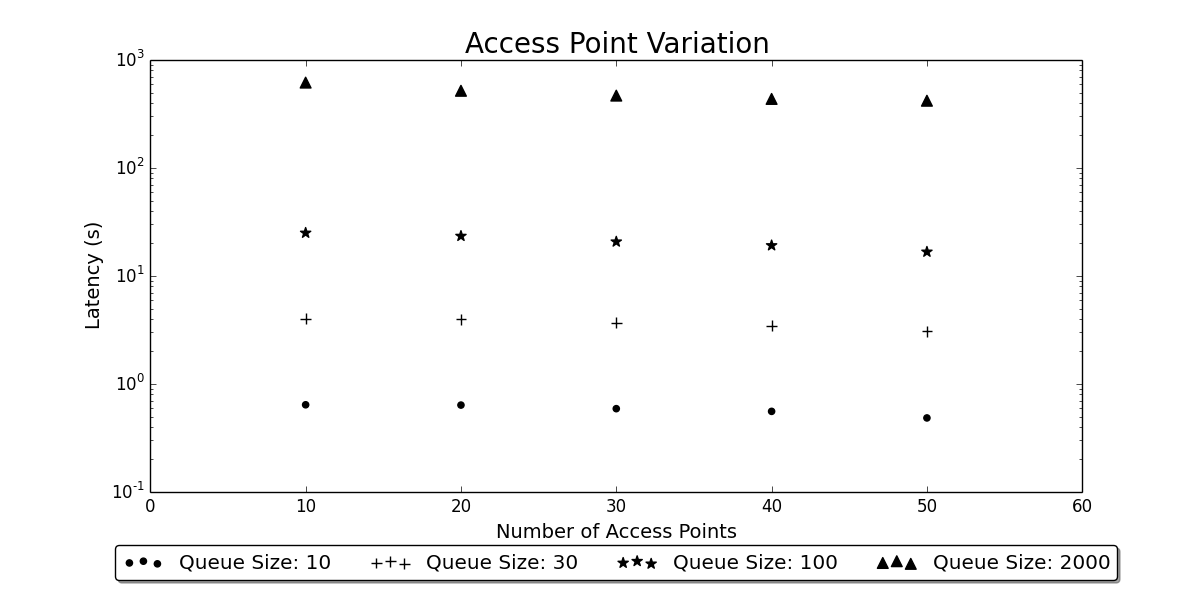
\includegraphics[width=\linewidth]{./images/Access_Point_Latency.png}
                \caption{}
                \label{fig:num_aps_latency}
            \end{subfigure}
            \begin{subfigure}{\textwidth}
                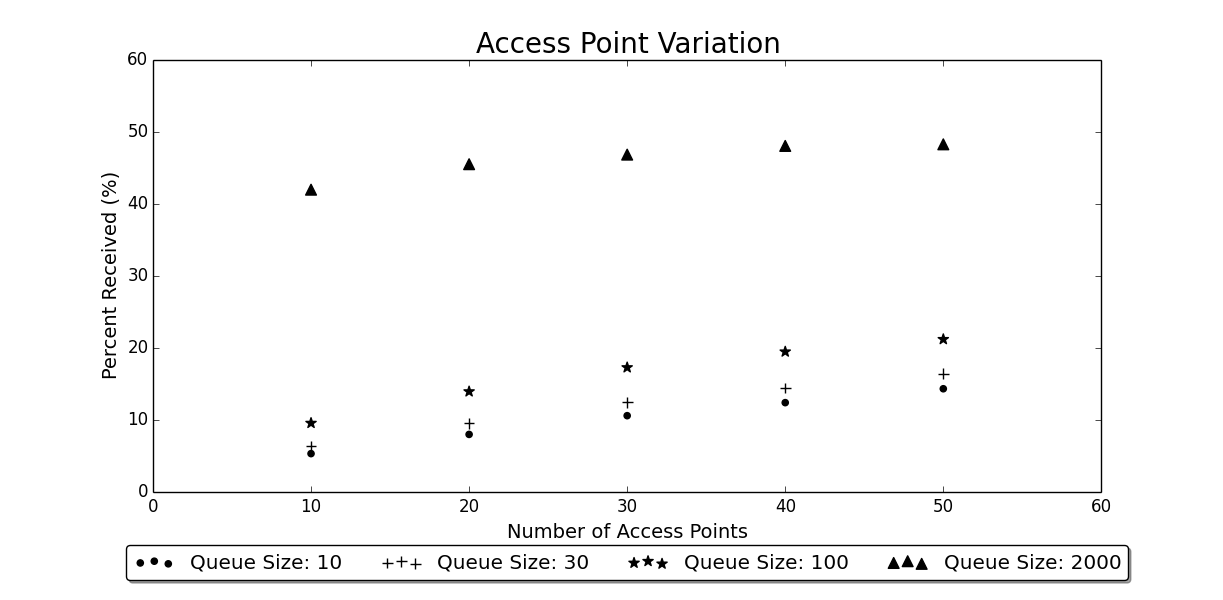
\includegraphics[width=\linewidth]{./images/Access_Point_Received.png}
                \caption{}
                \label{fig:num_aps_received}
            \end{subfigure}
            \caption{These figures show how the latency decreases with the number of APs (\ref{fig:num_aps_latency}), and the packet delivery rate increases (\ref{fig:num_aps_received}). (\ref{fig:num_aps_latency}) is plotted on a log scale in order to be able to differentiate between the various queue sizes.}
            \label{fig:num_aps}
        \end{figure}

        From this data we can see that the greater the number of APs, the lower the latency, and the greater the packet delivery rate. Once again we see that when adding a larger queue size the packet delivery rate increases but due to the extended storage time there is no improvement in latency, which manifests as a latency increase overall. When increasing the number of APs that disadvantage is no longer present. At smaller queue sizes we can double or even triple the packet delivery rate with more APs. It should be noted that as discussed in chapter~\ref{simulation} simulation time was one of the main factors for limiting the simulations to at most 50 APs. With the dataset we had over 2,000 APs which means we can expect a much greater packet delivery rate with a significantly lower mean latency in a physical implementation. 


    \section{Transmitter and Receiver Power}\label{data_gathering_performance_transmitter_and_reciever_power}

        A simple way of increasing the access point coverage of the city is to increase the power levels of the APs and receivers. This increase in power level causes them to serve a greater area without the need for any more APs. European legislation restricts all 2.4GHz radios to an equivalent isotropically radiated power level of 100mW~\cite{rackley2011wireless}, which when converted to dBm gives a value of 19.93dBm, or approximately 20dBm. In practice we cannot increase the power levels of the radios without breaking the law, however we can do this with a simulator and thereby study the effect of varying the power level in more detail. In order to determine the effect that power level has on the data collection performance we tested the model at 5 different power levels. These power levels were 18 dBm, 19 dBm, 20 dBm, 21 dBm and 22 dBm, which correspond to 64.00 mW, 80.63 mW, 101.59 mW, 128.00 mW and 161.27 mW respectively. Furthermore, we also must acknowledge that this is a simulation and therefore not identical to a physical implementation and so we need to understand that the propagation model will not be perfect. In order to find the most realistic model for our simulation we tried using 2 different models for this test. These propagation models were the Rayleigh model and the Log Normal Shadowing model. The results of this test, using a queue size of 2000 and all 50 APs, are shown in table~\ref{tab:power_level} and figure~\ref{fig:power_level}. 

        \afterpage{%
            \clearpage% Flush earlier floats (otherwise order might not be correct)
            \begin{landscape}
                \begin{table}
                    \centering
                    \begin{tabularx}{\linewidth}{|X|X|X|X|X|X|X|X|X|}
                        \hline
                        \multicolumn{1}{|X|}{\centering Power} & 
                        \multicolumn{1}{|X|}{\centering Model} & 
                        \multicolumn{1}{|X|}{\centering Mean \\ Latency (s)} & 
                        \multicolumn{1}{|X|}{\centering Standard \\ Deviation (s)} & 
                        \multicolumn{1}{|X|}{\centering Packets \\ Generated} & 
                        \multicolumn{1}{|X|}{\centering Packets \\ Sent} & 
                        \multicolumn{1}{|X|}{\centering Packets \\ Received} & 
                        \multicolumn{1}{|X|}{\centering Packets \\ Dropped} & 
                        \multicolumn{1}{|X|}{\centering \% \\ Received} \\
                        \hline
                        18 & Rayleigh & 154.12 & 323.82 & 294,743.60 & 522,092.80 & 238,455.20 & 1,986.40 & 80.74 \\
                        18 & Log Normal Shadowing & 122.62 & 278.35 & 279,041.50 & 452,601.00 & 225,997.50 & 2,268.75 & 79.72 \\
                        19 & Rayleigh & 128.94 & 281.37 & 270,759.00 & 473,615.20 & 213,552.20 & 933.20 & 78.72 \\
                        19 & Log Normal Shadowing & 169.79 & 363.87 & 527,232.75 & 868,566.75 & 431,838.25 & 34,279.50 & 83.15 \\
                        20 & Rayleigh & 150.13 & 322.72 & 299,218.50 & 525,681.25 & 240,421.75 & 1,445.50 & 80.26 \\
                        20 & Log Normal Shadowing & 150.72 & 316.18 & 470,629.50 & 782,219.50 & 388,500.00 & 20,491.00 & 81.03 \\
                        21 & Rayleigh & 116.22 & 255.51 & 220,911.00 & 383,434.50 & 169,469.00 & 0.00 & 76.79 \\
                        21 & Log Normal Shadowing & 86.43 & 203.14 & 179,300.00 & 290,371.00 & 134,968.00 & 0.00 & 75.27 \\
                        22 & Rayleigh & 135.75 & 294.37 & 270,957.00 & 471,525.67 & 218,749.33 & 977.33 & 80.54 \\
                        22 & Log Normal Shadowing & 0 & 0 & 0 & 0 & 0 & 0 & 0 \\
                        \hline
                    \end{tabularx}
                    \caption{The results of changing the power level of the radios.}
                    \label{tab:power_level}
                \end{table}
            \end{landscape}
        }

        \centerimage{0.7\linewidth}{./images/Power_Level.png}{A chart showing the small variations in latency and packet delivery when changing power level.}{fig:power_level}

        In terms of the propagation model a significant problem was found which may be apparent from the final row in table~\ref{tab:power_level}. There appeared to be a bug in the implementation in Omnet++ in which the simulation tended to crash when used with this simulation after some indeterminable period of time. Generally we did not get a simulation time of longer than 2,000 seconds which is significantly shorter than the 10,000 seconds we had been using previously. In some cases we did not get readings for particular runs using the Log Normal Shadowing model and therefore the mean result was made up of just 3 or 4 readings instead of 5. Furthermore, the effect that the software bugs had on the simulation when also trying the Log Normal Shadowing model also seemed to affect the simulation when using the Rayleigh model, which is the model used for all other experiments. As such no further experiments were performed on propagation models. 

        With the results we have we can still analyse the effect that power level has. The effect is almost non-existent. We would expect to see a decrease in latency and increase in packet delivery as the power level goes up, however we saw no such increase. It is theorised that the reason for this is that the packet upload time is dominated by the bandwidth of the connection. By increasing the power levels we may be in contact with an access point for an extra few seconds, however as we can upload 2000 packets in less than a second, which is an effective rate of approximately 47 KBps, this extra time only limits the delivery time of a single packet or two. Over a greater period of time, should the simulation not have crashed, it is possible that we may have seen a very small correlation, however it is insignificant at this time. 


    \section{Opportunistic Forwarding}\label{data_gathering_performance_opportunistic_forwarding}

        Air quality has been measured using vehicles before such as with the OpenSense project, however these project tend to rely on cellular connectivity for returning the data. Our system does not use cellular connectivity and instead relies on open WiFi APs. This method presents certain problems. The main problem being that we have no control over the location of these APs and as such buses may spend a long time out of range of an AP, or indeed may not even come into contact with one at all. Figure~\ref{fig:access_point_map} shows the locations of the 82 APs in Edinburgh we will be using for our simulations. We can see that these APs are clustered around the centre of the city and there are very few at distances of more than 2 miles from the centre. 

        \centerimagewideanywhere{./images/APMap.png}{A map of all 82 open APs which are used in our simulations. There is a faded red ring around the 2 mile mark from the city centre. This image uses \emph{Google Maps}.}{fig:access_point_map}

        From this image we can see that it is likely that we will run into issues should there be any buses which do not go through the city centre as part of their route. Unfortunately this is the case for at least one particular route. Buses on route 39 do not travel inside the city bypass at all, a boundary which is generally regarded as the bounds of the city. These buses travel around some of the villages in the south of the city. There are no recorded APs outside the city bypass. Route 39 is shown in figure~\ref{fig:route_39}.

        \centerimagewideanywhere{./images/Route39.png}{Lothian bus route 39. This image is taken from the Lothian Buses website and uses \emph{Google Maps}.}{fig:route_39}

        Based on the chemicals discuss in section~\ref{background_air_quality}, we know the data we need to store for each data packet. The total size of each packet is 24 bytes as shown by the packet composition in table~\ref{tab:data_packet}. Research in the first year of this project into creating a physical sensor revealed that the \emph{Arduino Uno} would make a good choice of base component. The reasons for this included its cost, size, and use in similar projects~\cite{arduinoproj1,arduinoproj2,arduinoproj3}. The Arduino Uno's main problem however is the limited space for storing data, with the standard version having just 32,256 bytes of storage space available~\cite{arduinounospecs}. This means that it can store at most 1,344 packets. With a new measurement every second this amounts to just over 22 minutes of data storage space. A more expensive version has storage space for 10,581 packets, which is just under 3 hours of recording. Ideally we would need at least one full days worth of storage space to ensure that all the recorded data makes it back to the central server since the buses return to a depot within the city at night should they not be in use and at least once a day to refuel. In order to ensure that we do not end up with only the last 22 minutes of data for the buses on route 39, or the last 22 minutes before finding an AP on routes which only have minimal access to APs, we need a different method of returning the data.

        \begin{table}
            \centering
            \begin{tabular}{ | c | c |}
                \hline
                Metric & Size (bytes)\\ \hline
                Timestamp & 4 \\
                Bus Id & 2 \\
                \cee{CO_{2}} & 2 \\
                \cee{NO_{x}} & 2 \\
                \cee{O_{3}} & 2 \\
                PM 10 & 2 \\
                PM 2.5 & 2 \\
                Latitude & 4 \\
                Longitude & 4 \\
                \hline
                Total & 24 \\
                \hline
            \end{tabular}
            \caption{The layout of a single data packet.}
            \label{tab:data_packet}
        \end{table}

        The solution for this is known as \emph{opportunistic forwarding}. Opportunistic forwarding consists of buses communicating with one another and passing the data between them so that as much data as possible will be returned to the central server with the lowest possible latency. An example of how this works can be shown using the buses on route 39. On this route there is a straight which the buses on route 40 also traverse. The buses on route 40 however travel into more densely populated areas and come into contact with APs. This can be seen in figure~\ref{fig:route_39_40}. When a bus on route 39 comes into contact with a bus on route 40, the buses exchange information about which will find an access point the soonest and the space they have available. In this case the bus on route 40 will come into contact with an AP first and so will accept the data from the route 39 bus. The bus on route 40 will accept as many packets as it can without causing it to lose any of its own between now and finding an AP. This is achieved by each bus being able to predict when it will come into contact with an AP. In reality this would be achieved by programming this buses with timetables and recording data about the APs they encountered, however since this data is unavailable to us, it is approximated with the current data set. Each bus knows about all 82 APs which are used, but each simulation only uses at most 50 of these. As such, buses may predict that they will encounter an AP which is not present in the simulation. This behaviour is representative of reality in that APs may be missing, however we would expect this to happen to a lesser extent in a physical implementation.

        \centerimagewideanywhere{./images/Route3940.png}{Lothian bus routes 39 (in blue) and 40 (in red). This image is taken from the Lothian Buses website and uses \emph{Google Maps}.}{fig:route_39_40}

        In a physical implementation of opportunistic forwarding, the standard mechanism would be to use a single radio and switch back and forth between the peer to peer communication mode and the AP detection mode. The reason for doing this is purely cost based. With a simulator we are not limited to this and as such we add a second radio in order to simplify implementation. The addition of a second radio would remove the fraction of a second delay to connecting to an AP when using a single radio, due to the context switch. However, as has been shown, the transfers are dominated by the bandwidth of the connection and so this should have a negligible effect. It also makes it more likely that broadcasts from other buses will be detected. It should be noted that in Omnet++, IP address allocation is a relatively complicated procedure when allocating addresses to more than 255 nodes and as such the decision was made to limit the number of allocated addresses to less than 255. Due to each bus having two radios we have only 125 buses in our opportunistic forwarding simulations, losing all buses from routes 5 and 37. This will have a slight negative effect on the performance of opportunistic forwarding, however due to time constraints the decision was made to continue with this method. The effects of removing buses are limited due to the buses being removed being constrained to specific routes. It is estimated that most opportunistic forwarding will occur between buses on the same route, heading in different directions. By removing entire routes, we should minimise the number of missed opportunistic forwards.

        The more important decision to be made is the algorithm which we will use in our model. Lebrun et al. discussed five different algorithms for opportunistic forwarding~\cite{opportunisticforwarding}. These algorithms were \emph{NOTALK}, \emph{BROADCAST}, \emph{Location-based}, \emph{MoVe} and \emph{MOVE-Lookahead}. NOTALK is the base case in which there is no communication between nodes and so will be discounted immediately. BROADCAST is the opposite in that every node exchanges information with every other node it comes into contact with. This method of routing is also known as \emph{epidemic routing}, and was first described by Vahdat et al. in~\cite{vahdat2000epidemic}. The goals and therefore advantages of epidemic routing, and therefore BROADCAST, as described by Vahdat et al. are ``i) maximize message delivery rate, ii) minimize message latency, and iii) minimize the total resources consumed in message delivery.'' Using opportunistic forwarding removes one of the main requirements of other routing algorithms which is the assumption that a path to an access point always exists. The price we pay for these advantages however is the large storage space requirements. Obviously this limitation is one which cannot be ignored due to the reasons discussed above and as so we must discount the BROADCAST algorithm. The MoVe and the MOVE-Lookahead algorithms require much more information than we have available and must also be discounted. This leaves us with one algorithm and that is the Location-based algorithm. This algorithm is derived from the BROADCAST algorithm by employing a heuristic. The heuristic is that the algorithm only passes on the data to the other sensor should it reach an access point first. This is the algorithm which was implemented in the simulation.

        The algorithm employs the following approach for the broadcasting bus, A:

        \begin{enumerate}
            \item Broadcast the first packet, appending metadata about the time until reaching an AP, in the queue to all nearby buses.
            \item If we receive a response to that packet, remove the packet from the queue and repeat.
            \item If we do not receive a response then try again in 0.5 seconds.
        \end{enumerate}

        For the receiving bus, B:

        \begin{enumerate}
            \item Compare the time until bus A will reach an AP to the time that this bus, B, will reach an AP using the metadata in the packet.
            \item If bus A reaches an AP first then discard this packet and do not respond.
            \item If bus B will reach an AP first then predict how much spare space bus B will have in its buffer when reaching the next AP:
                \begin{enumerate}
                    \item Calculate time until next AP, $t$.
                    \item Subtract $t$ from the space remaining in the queue, and call this result $s$.
                \end{enumerate}
            \item If $s$ is greater than 0 then accept this packet by adding it to our own queue and broadcasting a response.
        \end{enumerate}

        In order to successfully use this algorithm we need to provide extra information in our packets we send. This extra information includes the time until finding the next access point (4 bytes) and the identifier of the bus the packed \emph{originated} from (2 bytes). This addition of 6 bytes changes our packet size to 30 bytes in total. Which means that each device can no longer hold 1,344 packets and instead can only hold 1,075 packets, or in the case of the larger storage space it changes from 10,581 to 8,465. This is 18 minutes and 141 minutes of data respectively. 

        With the implementation discussed above, the best way to evaluate the performance is to run a simulation both with and without opportunistic forwarding. The results of this are shown in tables~\ref{tab:opportunistic_forwarding_first}, \ref{tab:opportunistic_forwarding} and figure~\ref{fig:opportunistic_forwarding}.

        \afterpage{%
            \clearpage% Flush earlier floats (otherwise order might not be correct)
            \begin{landscape}
                \begin{table}
                    \centering
                    \begin{tabularx}{\linewidth}{|X|X|X|X|X|X|X|X|X|X|X|}
                        \hline
                        \multicolumn{1}{|X|}{\centering Queue Size} & 
                        \multicolumn{1}{|X|}{\centering Mean Latency (s)} & 
                        \multicolumn{1}{|X|}{\centering Standard Deviation} & 
                        \multicolumn{1}{|X|}{\centering AP Received} & 
                        \multicolumn{1}{|X|}{\centering AP Unique} & 
                        \multicolumn{1}{|X|}{\centering Packets Sent} & 
                        \multicolumn{1}{|X|}{\centering Packets Successful} & 
                        \multicolumn{1}{|X|}{\centering Packets Stored} & 
                        \multicolumn{1}{|X|}{\centering Packets Dropped} \\
                        \hline
                        10 & 0.23 & 1.39 & 463,908 & 421,622 & 2,160,545 & 463,239 & 57,673 & 833,967 \\
                        30 & 1.52 & 5.96 & 626,482 & 499,921 & 2,200,064 & 598,384 & 128,859 & 759,144 \\
                        100 & 12.02 & 30.38 & 829,123 & 513,153 & 2,490,028 & 733,816 & 341,718 & 753,631 \\
                        1000 & 236.26 & 370.09 & 1,475,528 & 659,686 & 4,063,488 & 1,121,781 & 1,827,617 & 438,549 \\
                        2000 & 344.52 & 633.09 & 1,534,024 & 648,545 & 4,825,887 & 1,109,934 & 2,605,998 & 289,271 \\
                        \hline
                    \end{tabularx}
                \end{table}
                \begin{table}
                    \centering
                    \begin{tabularx}{\linewidth}{|X|X|X|X|X|X|X|X|X|X|X|}
                        \hline
                        \multicolumn{1}{|X|}{\centering Queue Size} & \multicolumn{1}{|X|}{\centering AP Received} & \multicolumn{1}{|X|}{\centering AP Unique} & \multicolumn{1}{|X|}{\centering Packets Sent} & \multicolumn{1}{|X|}{\centering Packets Successful} & \multicolumn{1}{|X|}{\centering Packets Stored} & \multicolumn{1}{|X|}{\centering Packets Dropped} & \multicolumn{1}{|X|}{\centering Queue Ignores Time} & \multicolumn{1}{|X|}{\centering Queue Ignores Space} & \multicolumn{1}{|X|}{\centering Queue Ignores Ratio} & \multicolumn{1}{|X|}{\centering \% Received} \\
                        \hline
                        10 & 463,908 & 421,623 & 2,160,545 & 463,239 & 57,673 & 833,967 & 8,183,045 & 8,567,042 & 0.955 & 33.73\% \\
                        30 & 626,482 & 499,921 & 2,200,064 & 598,384 & 128,859 & 759,144 & 7,126,313 & 7,348,423 & 0.975 & 39.99\% \\
                        100 & 829,123 & 513,153 & 2,490,028 & 733,816 & 341,718 & 753,631 & 8,189,153 & 8,429,989 & 0.971 & 41.05\% \\
                        1000 & 1,475,528 & 659,686 & 4,063,488 & 1,121,781 & 1,827,617 & 438,549 & 6,906,153 & 6,976,392 & 0.990 & 52.77\% \\
                        2000 & 1,534,025 & 648,545 & 4,825,887 & 1,109,934 & 2,605,998 & 289,271 & 5,808,998 & 5,644,930 & 1.030 & 51.88\% \\
                        \hline
                    \end{tabularx}
                    \caption{These two tables are part of the same table, split across the page. They show the results of using opportunistic forwarding.}
                    \label{tab:opportunistic_forwarding_first}
                    \begin{tabularx}{0.6\linewidth}{|X|X|X|X|X|}
                        \hline
                        \multicolumn{1}{|X|}{\centering Queue Size} & 
                        \multicolumn{1}{|X|}{\centering Non OF Latency (s)} & 
                        \multicolumn{1}{|X|}{\centering OF Latency (s)} & 
                        \multicolumn{1}{|X|}{\centering Non OF \% Received} & 
                        \multicolumn{1}{|X|}{\centering OF \% Received} \\
                        \hline
                        10 & 0.49 & 0.23 & 14.34 & 33.73 \\
                        30 & 3.08 & 1.52 & 16.43 & 39.99 \\
                        100 & 16.72 & 12.02 & 21.21 & 41.05 \\
                        1000 & - & 236.26 & - & 52.77 \\
                        2000 & 419.84 & 344.52 & 48.29 & 51.88 \\
                        \hline
                    \end{tabularx}
                    \caption{This table shows the packet delivery ratio of using opportunistic forwarding versus not using opportunistic forwarding.}
                    \label{tab:opportunistic_forwarding}
                \end{table}
            \end{landscape}
        }

        \begin{figure}
            \centering
            \begin{subfigure}{0.5\textwidth}
                \centering
                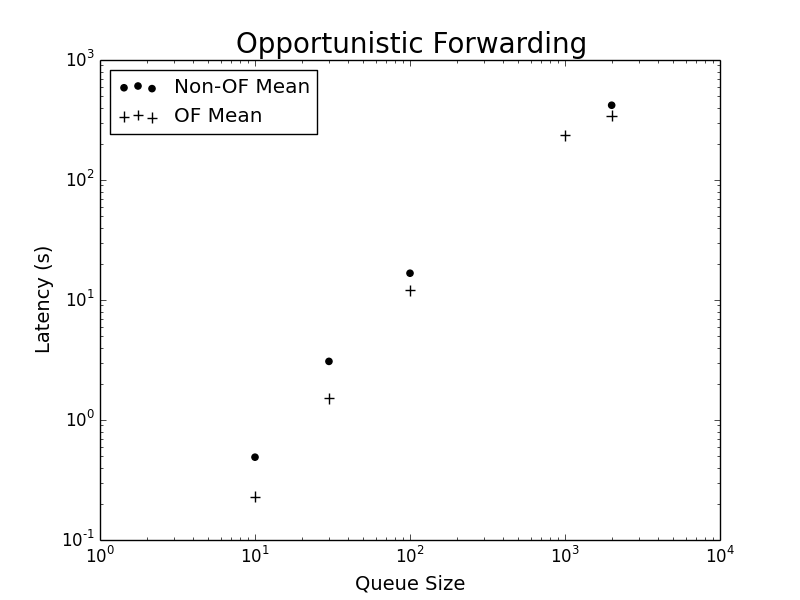
\includegraphics[width=\linewidth]{./images/OF_Latency.png}
                \caption{}
                \label{fig:of_latency}
            \end{subfigure}%
            \begin{subfigure}{0.5\textwidth}
                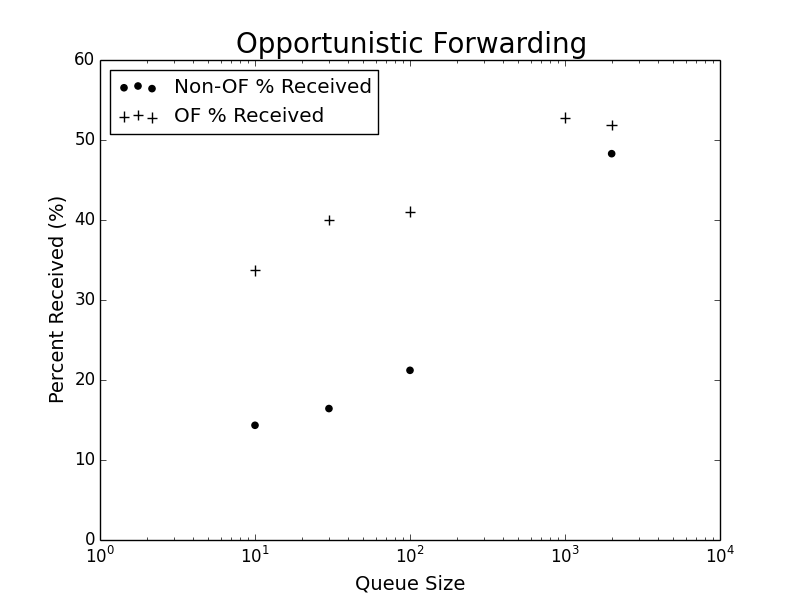
\includegraphics[width=\linewidth]{./images/OF_Received.png}
                \caption{}
                \label{fig:of_recieved}
            \end{subfigure}
            \caption{These figures show how the latency decreases when using opportunistic forwarding (OF) (\ref{fig:of_latency}), and the packet delivery rate increases (\ref{fig:of_recieved}). Note that (\ref{fig:of_latency}) is on a log scale.}
            \label{fig:opportunistic_forwarding}
        \end{figure}

        With opportunistic forwarding, the same pattern is followed as with no opportunistic forwarding. When we increase the queue size, the packet delivery rate goes up, as does the latency. The interesting part is when we compare the two results. This is seen in table~\ref{tab:opportunistic_forwarding} and figure~\ref{fig:opportunistic_forwarding}. The results clearly show that using opportunistic forwarding increases the efficiency of our system. At low queue sizes, such as 10, it more than doubles the packet delivery ratio while also halving the mean latency. As we move to larger queue sizes the effect becomes less pronounced. With a queue size of 2000 we only increase the packet delivery rate from 48.29\% to 51.88\%, however the average latency of a packet is over a minute less at just 344.5 seconds compared to 419.8 seconds. While the results seem to converge, it is unclear at this point if opportunistic forwarding would ever cause a detrimental effect to the results and requires further study.


    \subsection{Non-Chronological Queue}\label{data_gathering_performance_non-chronological_queue}

        Due to the apparent convergence of the results when using opportunistic forwarding a modification to the algorithm was proposed. In the initial runs, when bus $a$ received a packet from bus $b$ it would look at the time stamp on the packet from $b$ and use this to insert it into its own queue at the correct chronological point. That is to say the queue of packets maintained by each bus is always in a strict monotonic chronological order based on the packet generation time. In order to tell if any effects are caused because of this decision the same simulations as in section~\ref{data_gathering_performance_opportunistic_forwarding} were run once again, with the modification that any packets that $a$ receives from any other bus are simply placed at the tail end of the queue. The results of this compared to the original time stamp queued version are presented in table~\ref{tab:priority_queue} and figure~\ref{fig:priority_queue}.

        \begin{table}[H]
            \begin{tabularx}{\linewidth}{|X|X|X|X|X|}
                \hline
                \multicolumn{1}{|X|}{\centering Queue Size} & 
                \multicolumn{1}{|X|}{\centering Chronological Latency (s)} & 
                \multicolumn{1}{|X|}{\centering Non-Chronological Latency (s)} & 
                \multicolumn{1}{|X|}{\centering Chronological \% Received} & 
                \multicolumn{1}{|X|}{\centering Non-Chronological. \% Received} \\
                \hline
                10 & 0.23 & 0.20 & 33.73 & 37.71 \\
                30 & 1.52 & 1.00 & 39.99 & 38.67 \\
                100 & 12.02 & 6.98 & 41.05 & 42.75 \\
                1000 & 236.26 & 184.07 & 52.77 & 58.86 \\
                2000 & 244.52 & 373.48 & 51.88 & 65.60 \\
                \hline
            \end{tabularx}
            \caption{This table shows the packet delivery ratio of using opportunistic forwarding with the original queue based on time stamp  and the non-chronological version which appends all received packets to the queue.}
            \label{tab:priority_queue}
        \end{table}

        \begin{figure}
            \centering
            \begin{subfigure}{0.5\textwidth}
                \centering
                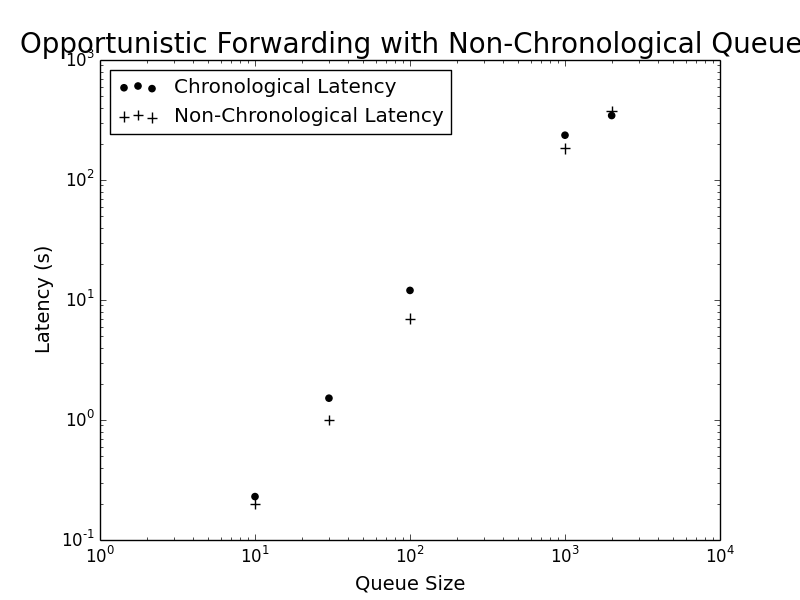
\includegraphics[width=\linewidth]{./images/OF_Non_Chron_Latency.png}
                \caption{}
                \label{fig:of_non_chron_latency}
            \end{subfigure}%
            \begin{subfigure}{0.5\textwidth}
                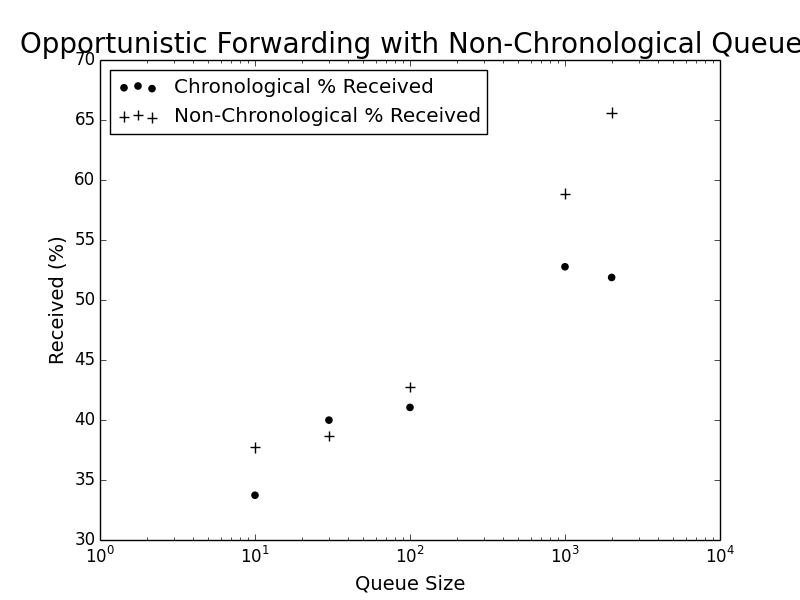
\includegraphics[width=\linewidth]{./images/OF_Non_Chron_Received.png}
                \caption{}
                \label{fig:of_non_chron_received}
            \end{subfigure}
            \caption{These figures show how the latency decreases when using a non-chronological queue with opportunistic forwarding (OF) (\ref{fig:of_non_chron_latency}), and the packet delivery rate increases (\ref{fig:of_non_chron_received}). Note that (\ref{fig:of_non_chron_latency}) is on a log scale.}
            \label{fig:priority_queue}
        \end{figure}

        The results from this show that at smaller queue sizes, that is 10-1000 packets, the latency is even lower when simply appending to the end of the queue. At all measured queue sizes, with the exception of 30 which may be a statistical anomaly, the packet delivery rate is significantly improved. However, at higher queue sizes, i.e. 2000 onwards, it seems that this advantage is diminished by the increased latency, however, as we have discussed in previous sections, the price paid for holding onto more packets for longer in order to ensure they are delivered is that the latency will increase. 

        The unexpected effect is that appending to the end of the queue instead of inserting into the correct position has a positive effect on the delivery ratio. While we may expect this to have no change at all, the effect is due to duplication of packets. If a bus, $a$, broadcasts a packet and there are 4 buses in the immediate vicinity who accept the packet then we have 4 duplicates. Bus $a$ will receive a response and then move on to broadcasting the next packet in the queue, ignoring that 4 buses have the packet now. When a bus gets a full queue from a miscalculation of when it will encounter an AP, or for any other reason, it drops the packets at the front of the queue. In the chronological queue version where we insert packets at the correct chronological position, the oldest packets are penalised and since the duplicates all have the same time stamp they will tend to all be dropped, rather than the unique packets that the buses carry. 

        When we compare this result to the base line, as in table~\ref{tab:opportunistic_queue_good} and figure~\ref{fig:opportunistic_queue_good}, without opportunistic forwarding, the results are striking. With a queue size of 10 we get 163\% and 145\% better performance in terms of packet delivery and latency respectively. With the largest queue size of 2,000 we get an increase of 37\% and 12\% in terms of packet delivery and latency respectively. Again, it seems like these two series will converge, but not until we reach 100\% packet delivery, which is equivalent to no convergence.

        \begin{table}
            \centering
            \begin{tabularx}{0.8\linewidth}{|X|X|X|X|X|}
                \hline
                \multicolumn{1}{|X|}{\centering Queue Size} & 
                \multicolumn{1}{|X|}{\centering Non OF Latency (s)} & 
                \multicolumn{1}{|X|}{\centering OF Latency (s)} & 
                \multicolumn{1}{|X|}{\centering Non OF \% Received} & 
                \multicolumn{1}{|X|}{\centering OF \% Received} \\
                \hline
                10 & 0.49 & 0.20 & 14.34 & 37.71 \\
                30 & 3.08 & 1.00 & 16.43 & 38.67 \\
                100 & 16.72 & 6.98 & 21.21 & 42.75 \\
                1000 & - & 184.07 & - & 58.86 \\
                2000 & 419.84 & 373.48 & 48.29 & 65.60 \\
                \hline
            \end{tabularx}
            \caption{This table shows the packet delivery ratio of using opportunistic forwarding versus not using opportunistic forwarding.}
            \label{tab:opportunistic_queue_good}
        \end{table}
        
        \begin{figure}
            \centering
            \begin{subfigure}{0.5\textwidth}
                \centering
                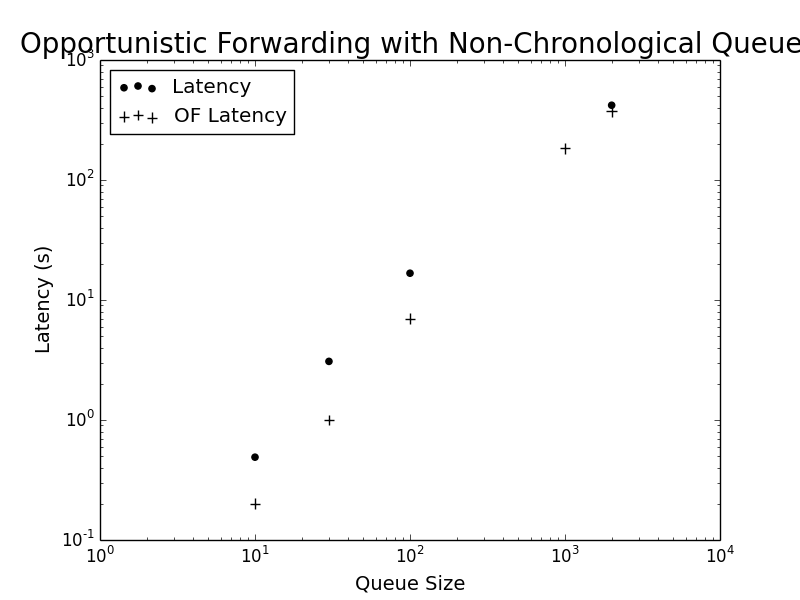
\includegraphics[width=\linewidth]{./images/OF_Complete_Latency.png}
                \caption{}
                \label{fig:of_complete_latency}
            \end{subfigure}%
            \begin{subfigure}{0.5\textwidth}
                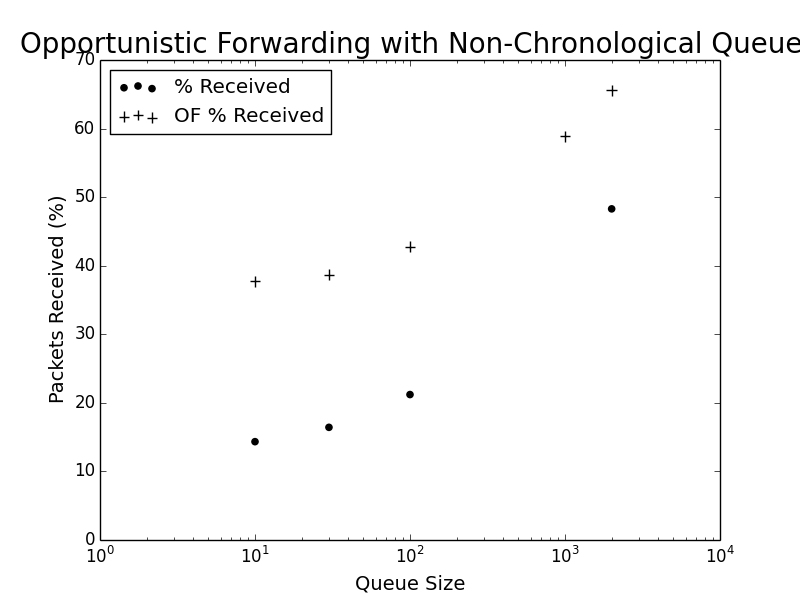
\includegraphics[width=\linewidth]{./images/OF_Complete_Received.png}
                \caption{}
                \label{fig:of_complete_received}
            \end{subfigure}
            \caption{These figures compare opportunistic forwarding with a non-chronological queue against the results of simulations where opportunistic forwarding is not used. They show how the latency decreases when using opportunistic forwarding (OF) (\ref{fig:of_complete_latency}), and the packet delivery rate increases (\ref{fig:of_complete_received}). Note that (\ref{fig:of_complete_latency}) is on a log scale.}
            \label{fig:opportunistic_queue_good}
        \end{figure}

    \subsection{Number of Access Points}\label{data_gathering_performance_number_of_access_points}

        In order to test the relative efficiency of the opportunistic forwarding algorithm a simulation was run with varying numbers of APs. In doing this we can find the number of APs which are required when using opportunistic forwarding to equal the performance of the non-opportunistic forwarding algorithm using fifty APs. The simulation was run with five different queue sizes and give different numbers of APs. It was determined with some preliminary tests that twenty-five was the approximate cross over point as as such the number of APs tested were 15, 20, 25, 30 and 35. However, upon completion of the simulation and the aggregation of the results, it was clear that the initial check was a statistical anomaly. When charting the latency, seen in figure~\ref{fig:of_num_aps_latency}, we can see that the actual cross over point, that is to say the number of APs with opportunistic forwarding which matches the performance of no opportunistic forwarding with 50 APs, is closer to 10 APs. When we look at the percentage of packets delivered, figure~\ref{fig:of_num_aps_percentage} the results are even more pronounced, with a queue size of 10 and 15 APs performing better than a queue size of 100 and 50 APs when not using opportunistic forwarding.

        \begin{figure}
            \centering
            \begin{subfigure}{0.5\textwidth}
                \centering
                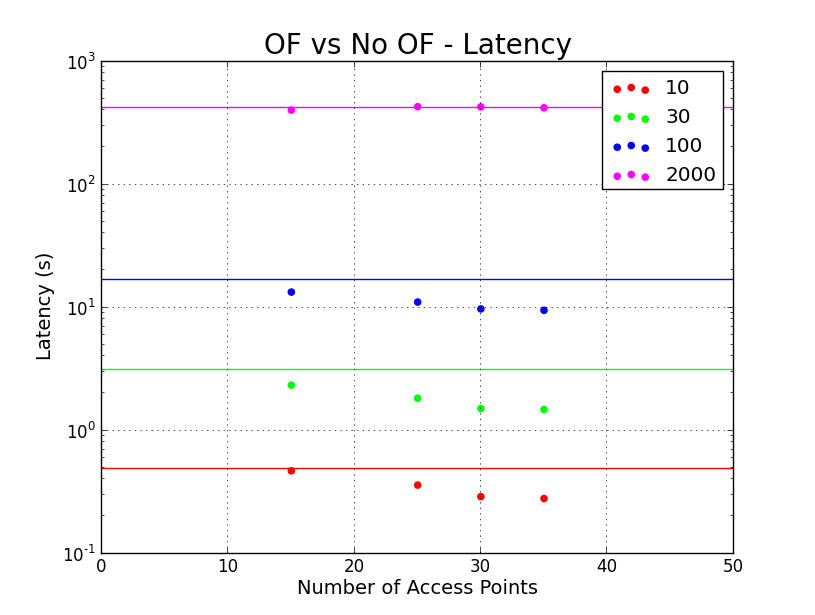
\includegraphics[width=\linewidth]{./images/OF_vs_No_OF_Latency.png}
                \caption{}
                \label{fig:of_num_aps_latency}
            \end{subfigure}%
            \begin{subfigure}{0.5\textwidth}
                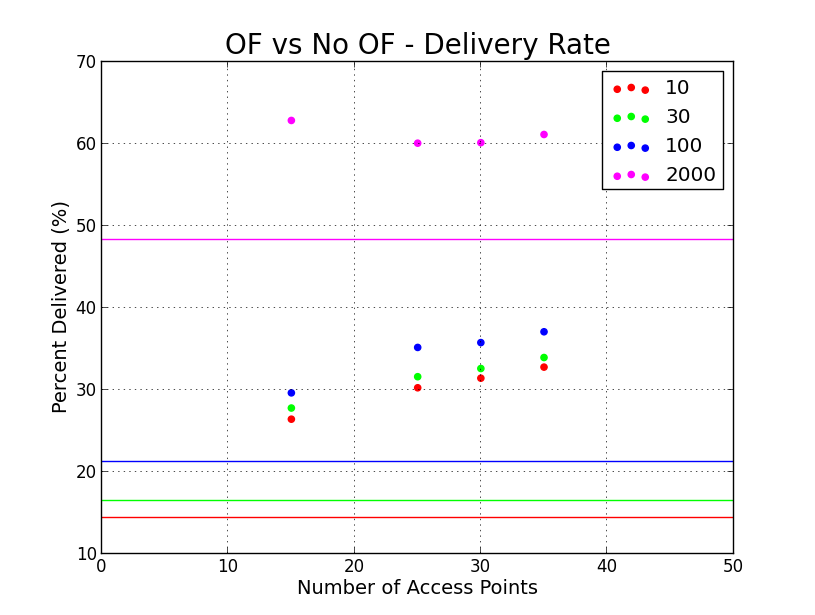
\includegraphics[width=\linewidth]{./images/OF_vs_No_OF_Percentage.png}
                \caption{}
                \label{fig:of_num_aps_percentage}
            \end{subfigure}
            \caption{These figures compare the algorithm without opportunistic forwarding and 50 APs against the opportunistic algorithm with a varying number of APs. The results without opportunistic forwarding are denoted by the coloured lines, with the corresponding queue sizes with opportunistic forwarding having corresponding colours. Please note that the data points for 20 APs are missing due to a hardware fault which caused a loss of data.}
            \label{fig:of_num_aps}
        \end{figure}


    \section{Conclusions}\label{data_gathering_performance_conclusions}

        Some of the information we have learned from the simulation was expected, such as increasing the number of APs increases packet delivery and reduces latency, however some of it is unexpected. Increasing the queue size causing an increase in latency was not an obvious result before hand, however it has made it clear that there is a trade off between packet delivery rates and packet latency. It was also found that, surprisingly, transmitter and receiver power had almost no effect on the results due to the connection speed dominating the small increase in transmission distance, theorised to be caused by the transmission speed dominating the other factors.

        The most effective optimisation was the introduction of opportunistic forwarding. When using the non-chronological version of the queuing mechanism the results are extremely promising. We also found that we can use many fewer APs when using opportunistic forwarding and achieve comparable performance to non-opportunistic forwarding examples, with 15 APs and opportunistic forwarding achieving better performance than 50 APs without opportunistic forwarding, for all queue sizes tested. The implications of this are the greatest. It illustrates that it may be possible to use such a system in a more rural setting, one where there is much poorer coverage of WiFi APs, unfortunately in such a scenario we would likely have fewer buses, and the effects of fewer buses have yet to be determined. 

        While the results are promising, we also must address the nature of the method of acquiring the results. Simulation, by its nature, requires that we use approximations in some areas. Due to this, we cannot confirm that in reality the model would behave exactly as the above results dictate. However, due to the use of an advanced networking simulator, the results should be representative of reality. One of the key issues with the simulation, which would cause our results to improve, is that the simulation treats Edinburgh as a two dimensional map, which results in there being no concept of terrain or buildings. The simulation assumes that there is line of sight between the sensors and the APs, however this is unlikely to always be the case. The APs will also be in buildings, a fact which has already partially been taken into account with the simulation as we had information about relative signal strength, and may be blocked by other structures and vehicles. 

        Despite the flaws above, these results are very reasonable, and combined with the knowledge we learned, that increasing the number of APs is beneficial to both the latency and packet delivery, it is likely that with the 2,000 known APs around the city, we would almost certainly see even better results.

